\documentclass[../main.tex]{subfiles}

\begin{document}

En esta sección se van a hacer dos posibles consultas que harían distintos usuarios a la base de datos, para lo que se usan las queries o consultas. Una consulta sirve encontrar y extraer elementos y atributos de una base de datos.

\hfill

Para realizar estas consultas se va a usar XQuery, un lenguaje para realizar consultas en documentos XML. Se basa en funciones, expresiones XPath y predicados.

\hfill

Las operaciones más comunes para hacer queries son SELECT, que selecciona los datos que serán visibles en la tabla resultado; FROM, para señalar la o las tablas de las cuales quiero obtener la información, WHERE, utilizada para delimitar la información que queremos obtener.

\subsection{Query 1}

Se procede a implementar una xquery que devuelve el número de estudios de 2012 sobre un antibiótico dado, para ello se declara una variable con el número de estudios que tengan estas características.

\begin{figure}[ht]
    \centering
    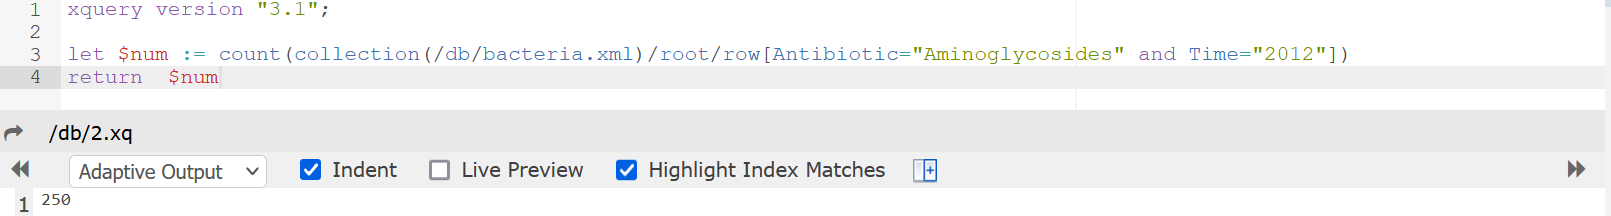
\includegraphics[width=0.95\textwidth]{images/xq1.png}
    \caption{XQuery 1}
    \label{xq1}
\end{figure}

\newpage

\subsection{Query 2}

Se procede a implementar una xquery que devuelva el nombre de los antibióticos de estudios de 2014 que tengan un valor superior al 50 por ciento

\begin{figure}[ht]
    \centering
    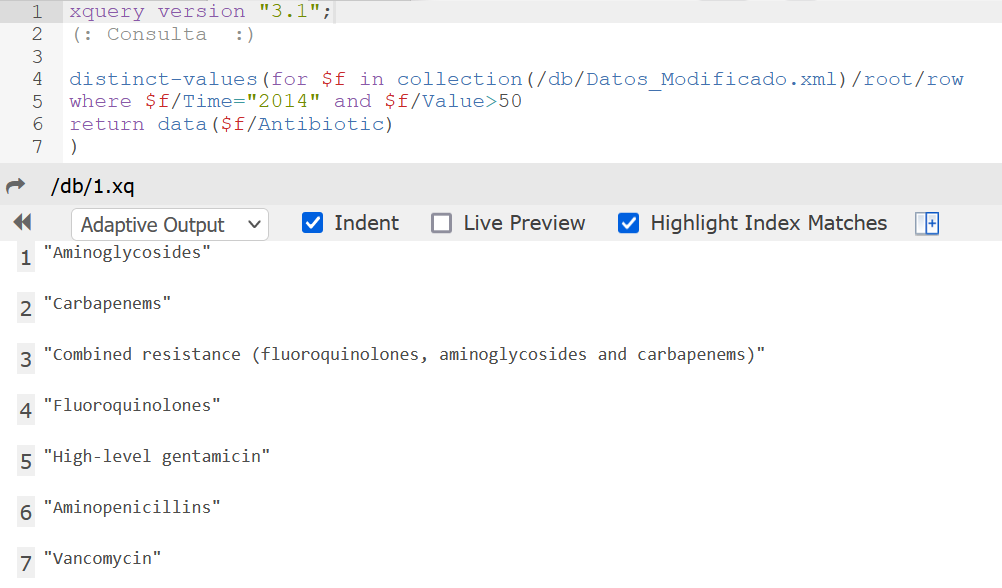
\includegraphics[width=0.95\textwidth]{images/xq2.png}
    \caption{XQuery 2}
    \label{xq2}
\end{figure}

\end{document}